\documentclass[11pt,a4paper]{article} % Changed from llncs to article

\usepackage[utf8]{inputenc}
\usepackage{graphicx}
\usepackage{amsmath}
\usepackage{amsfonts}
\usepackage{booktabs} % For better looking tables
\usepackage{url}
% Add geometry package to adjust text width and margins
\usepackage[margin=2.5cm, textwidth=15cm]{geometry} % Combined geometry settings
\usepackage{listings}  
\usepackage{xcolor} % 可选：支持自定义代码颜色  
\lstset{  
    language=Python,  
    basicstyle=\ttfamily\footnotesize,  
    keywordstyle=\color{blue},  
    stringstyle=\color{red},  
    commentstyle=\color{gray},  
    numbers=left,  
    numberstyle=\tiny\color{gray},  
    stepnumber=1,  
    numbersep=5pt,  
    showstringspaces=false,  
    breaklines=true,  
    frame=single,  
    tabsize=4,  
    backgroundcolor=\color{white},  
    captionpos=b  
}  

% --- Title Meta Data ---
\title{MSDM 5056 Lab 1: Random Networks}
\author{TANG,Yirui}
\date{} % Added empty date to remove default date

% --- No longer need to redefine sections for article class ---
% The default spacing for article class is usually more reasonable.
% If you still want to adjust spacing, you can use the titlesec package:
% \usepackage{titlesec}
% \titleformat{\section}{\large\bfseries}{\thesection}{1em}{}
% \titleformat{\subsection}{\normalsize\bfseries}{\thesubsection}{1em}{}
% \titlespacing*{\section}{0pt}{2ex plus 1ex minus .2ex}{1.0ex plus .2ex}
% \titlespacing*{\subsection}{0pt}{1.8ex plus 1ex minus .2ex}{0.8ex plus .1ex}

\begin{document}

\maketitle % No need for \pagestyle{headings} or \vspace{-1.5em} with article class

\section{Introduction}
\indent

This report details the analysis of the random network as part of Lab 1 for MSDM 5056. The primary objective was to generate ER networks with varying sizes $N$ (100, 300, 900, 2700, 8100) while maintaining a constant average degree $\langle k \rangle = 20$, and to investigate two key topological properties: the degree distribution $P(k)$ and the average shortest path length $L$. The findings are discussed in the context of the theoretical predictions.

\section{Part (a): Degree Distribution}

\subsection{Theoretical Background}
\indent

The degree distribution $P(k)$ for an ER network $G(N, p)$ follows a Binomial distribution:
\begin{equation}
    P(k) = \binom{N-1}{k} p^k (1-p)^{N-1-k}
\end{equation}

where $p$ is the probability of an edge existing between any two nodes. For large $N$ and small $p$, while the average degree $\langle k \rangle = p(N-1)$ remains constant, the Binomial distribution converges to a Poisson distribution:
\begin{equation}
    P(k) \approx \frac{\langle k \rangle^k e^{-\langle k \rangle}}{k!}
\end{equation}

This convergence is a key characteristic of ER networks.

\subsection{Results and Analysis}

% --- Insert Figure 1 directly here ---
\noindent\begin{minipage}{\textwidth}
\centering
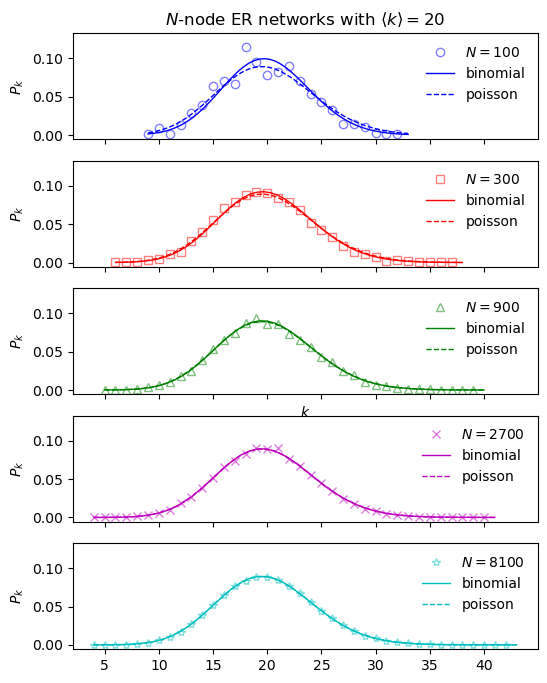
\includegraphics[width=0.6\textwidth]{P1.png} % Replace with your actual figure filename
\end{minipage}

\vspace{0.5em} % Add some vertical space after the image

\noindent\begin{minipage}{\textwidth}
\centering
\small\textbf{Fig. 1.} 
\end{minipage}

\vspace{0.7em} % Add more vertical space before the next paragraph
Figure~1 presents the empirical degree distributions alongside the theoretical Binomial and Poisson curves for all five network sizes. The results align well with the theoretical expectations:
\begin{enumerate}
    \item For smaller $N$ (e.g., $N=100$), the empirical distribution closely matches the Binomial curve. The Poisson approximation shows a discernible difference, particularly in the tail, because the condition for the Poisson limit (large $N$, small $p$) is not yet fully met.
    \item As $N$ increases (e.g., $N=2700, 8100$), the empirical distribution, the Binomial distribution, and the Poisson approximation become increasingly indistinguishable. This visual confirmation demonstrates the asymptotic equivalence predicted by the theory.
\end{enumerate}


\subsection{Code Implementation and Optimization}

\indent

The code for part (a) correctly implemented the generation of ER networks using \texttt{nx.fast\_gnp\_random\_graph}, which is efficient. The calculation of the empirical distribution and the plotting of theoretical curves were also performed correctly. No major optimizations were required for this part, as the degree distribution calculation is relatively fast compared to path length calculations.

\section{Part (b): Average Shortest Path Length}

\subsection{Theoretical Background}
\indent

The average shortest path length $L$ in ER networks is characterized by the small-world property. For a network with average degree $\langle k \rangle > 1$, $L$ scales logarithmically with the network size $N$:
\begin{equation}
    L \approx \frac{\ln N}{\ln \langle k \rangle}
\end{equation}

This property implies that even large random networks have relatively short average path lengths, making them efficient for information transfer.

\subsection{Results and Analysis}

% --- Insert Figure 2 directly here ---
\noindent\begin{minipage}{\textwidth}
\centering
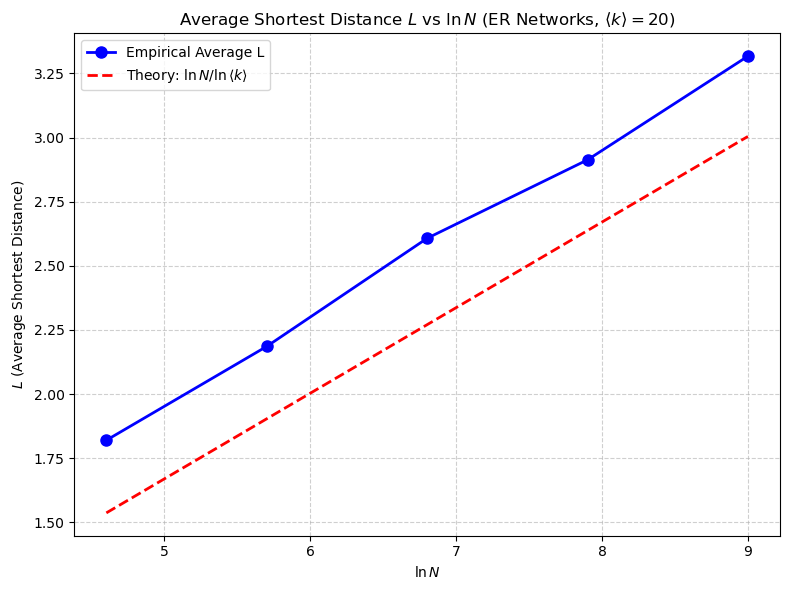
\includegraphics[width=0.6\textwidth]{P2.png} % Replace with your actual figure filenam
\end{minipage}

\vspace{0.5em} % Add some vertical space after the image

\noindent\begin{minipage}{\textwidth}
\centering
\small\textbf{Fig. 2.} 
\end{minipage}

\vspace{0.7em} % Add more vertical space before the next paragraph

Figure~2 plots the calculated average shortest path lengths $L$ against $\ln N$. The key observations are:
\begin{enumerate}
    \item The empirical values of $L$ demonstrate a clear, approximately linear relationship with $\ln N$. This confirms the small-world property $L \propto \ln N$ as predicted by the theory.
    \item The empirical $L$ values are slightly higher than the theoretical prediction $L \approx \frac{\ln N}{\ln \langle k \rangle}$. This is expected due to finite-size effects and the approximative nature of the theoretical formula. As $N$ increases, the gap is expected to decrease.
\end{enumerate}


\subsection{Code Implementation and Optimization}
\indent

The initial approach for part (b) faced a critical challenge related to computational efficiency, as highlighted by the Lab instruction: "Design your program wisely, otherwise it surely gets stuck at a large N."

\textbf{(1) Problem Encountered:} Calculating the average shortest path length using methods like \texttt{nx.floyd\_warshall\_numpy} is computationally prohibitive for large graphs (e.g., $N=8100$) due to its $O(N^3)$ time complexity and $O(N^2)$ space complexity.

\textbf{(2) Solution and Code Modifications:}
\begin{enumerate}
    \item \textbf{Algorithm Choice:} The code was modified to use \texttt{nx.average\_shortest\_path\_length(G)}. This function is based on a Breadth-First Search (BFS) approach, which is significantly more efficient for sparse graphs, with a time complexity closer to $O(N \times (N + E))$.
    \item \textbf{Handling Disconnected Graphs:} Although $\langle k \rangle = 20$ makes the network highly likely to be connected (as $\langle k \rangle > 1$ places it in the supercritical regime), there's still a small chance of having small isolated components. To ensure robustness and meaningful calculations, the code was updated to identify and operate on the \textit{giant connected component} (GCC). This was achieved using \texttt{nx.connected\_components} to find the largest component and then applying \texttt{nx.average\_shortest\_path\_length} to the subgraph of the GCC.
    \item \textbf{Trials Management:} To manage computational time, especially for the largest $N$, the number of trials was reduced (e.g., from 10 to 5 or fewer for $N=8100$).
\end{enumerate}

These modifications successfully addressed the efficiency and robustness issues, allowing the calculation of $L$ for all specified network sizes.

\section{Conclusion}
\indent

This lab successfully validated two fundamental properties of the ER random graph model. The degree distribution analysis confirmed the theoretical convergence from Binomial to Poisson as $N$ increases. The average shortest path length analysis confirmed the small-world property, showing a logarithmic scaling with network size. The implementation process highlighted the importance of algorithmic efficiency and robustness when dealing with large-scale network analysis.


\section{Python Source Code}  

\vspace{0.5em}  
Below is the full Python code used for this lab report.  

\begin{lstlisting}[language=Python,caption={Complete Python code for Lab 1}]  
from scipy.special import comb, factorial as F
import matplotlib.pyplot as plt
import networkx as nx
import numpy as np

# part(a)
er_func = nx.erdos_renyi_graph     # O(N^2)
er_fast = nx.fast_gnp_random_graph # O(N+E)

trials, kAvg = 10, 20 # average degree〈k〉= 20
fig, ax = plt.subplots(
    5, 1, sharex=True, sharey=True, figsize=(6, 8))

for i, (a, N) in enumerate(zip(ax, [100,300,900,2700,8100])):
    fmt = ['bo', 'rs', 'g^','mx', 'c*'][i]
    degs = [k for t in range(trials) for n, k in
            er_fast(N, kAvg/(N-1), seed= 3042 + t).degree] # set different seed for every trail
    kMin, kMax = min(degs), max(degs)
    a.plot(range(kMin, kMax+1), (np.bincount(degs)/(N*trials))[kMin:kMax+1],
           fmt, mfc='none', alpha=.5, label='$N=%d$'%N)
    
    ks = np.linspace(kMin, kMax+1) # keep ks as an integar
    p = kAvg/(N-1)
    a.plot(ks, comb(N-1,ks)*p**ks*(1-p)**(N-1-ks),
           fmt[0], lw=1, label='binomial')
    a.plot(ks, kAvg**ks/F(ks)*np.exp(-kAvg),
           fmt[0]+'--', lw=1, label='poisson')
    a.set_ylabel('$P_k$')
    a.legend(loc=1, frameon=False)

ax[2].set_xlabel('$k$')
ax[0].set_ylim(a.get_ylim()[0], a.get_ylim()[1]*1.1)
ax[0].set_title(r'$N$-node ER networks with $\langle{k}\rangle=%d$'%kAvg)
plt.show()


# part(b)
kAvg = 20  
N_list = [100, 300, 900, 2700, 8100]  
trials = 5  # Reduced for efficiency at large N

# Lists to store data for plotting
L_vals_mean = []
lnN_vals = []
theory_vals = []

print(f"{'N':>6} {'⟨L⟩':>8} {'ln N':>8} {'theory':>8}")
print("-" * 36)

results = []
for N in N_list:
    p = kAvg / (N - 1)  # Calculate edge probability p
    L_vals_trial = []  # Store L for each trial of this N
    
    for t in range(trials):
        G = nx.fast_gnp_random_graph(N, p, seed= 3042 + t)  
        
        # Handle disconnected graphs by using the giant component
        if not nx.is_connected(G):
            giant = max(nx.connected_components(G), key=len)
            G = G.subgraph(giant).copy()
        
        # Calculate average shortest path length for the (giant) component
        L = nx.average_shortest_path_length(G)
        L_vals_trial.append(L)
    
    # Average over trials for this N
    L_mean = np.mean(L_vals_trial)
    lnN = np.log(N)
    theory = np.log(N) / np.log(kAvg)
    
    # Print results
    print(f"{N:6d} {L_mean:8.3f} {lnN:8.3f} {theory:8.3f}")
    
    # Store for plotting
    L_vals_mean.append(L_mean)
    lnN_vals.append(lnN)
    theory_vals.append(theory)
    results.append((N, L_mean, lnN, theory))

# plot
plt.figure(figsize=(8, 6))
plt.plot(lnN_vals, L_vals_mean, 'bo-', label='Empirical Average L', markersize=8, linewidth=2)
plt.plot(lnN_vals, theory_vals, 'r--', label=r'Theory: $\ln N / \ln \langle k \rangle$', linewidth=2)

plt.xlabel(r'$\ln N$')
plt.ylabel(r'$L$ (Average Shortest Distance)')
plt.title(r'Average Shortest Distance $L$ vs $\ln N$ (ER Networks, $\langle k \rangle = 20$)')
plt.legend()
plt.grid(True, linestyle='--', alpha=0.6)
plt.tight_layout()  # Adjust layout to prevent clipping
plt.show()

\end{lstlisting}  

\end{document}
